\section{Platform}

\subsection{The workflow}

This section describes a platform that was designed to support a possible, general-purpose hybrid human-machine workflow for the creation and curation of geospatial data, attempting to address the challenges described in \ref{challenges-of-crowdsourcing-geospatial-data}. The workflow is shown in Figure \ref{fig:workflow_0}.

\begin{figure}
	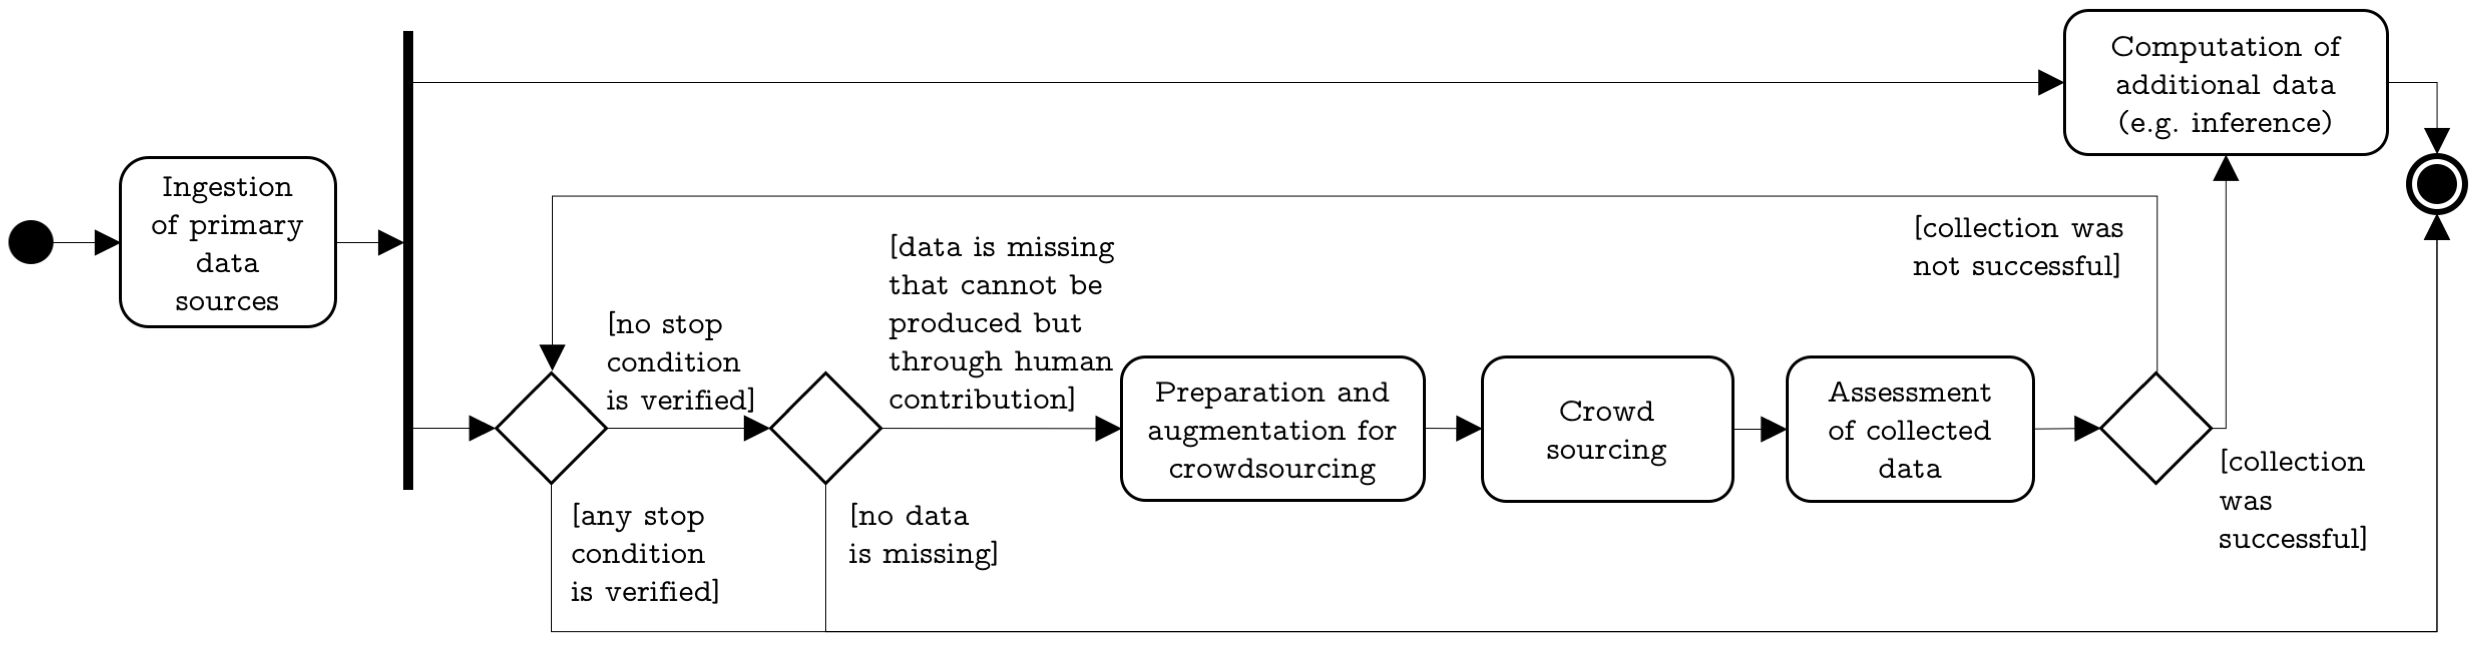
\includegraphics[width=1.0\textwidth]{workflow-0.png}
	\caption{General workflow}
	\label{fig:workflow_0}
\end{figure}

\subsection{Overall design principles}

The platform was designed following the principles below:

\textbf{Human-machine workflows support} The platform meant to automate as much as possible of the data creation / curation process, while effectively integrating human components, from administration to the crowdsourcing of part.

\textbf{Data re-use} As mentioned in chapter \ref{open-data-and-gi} we wanted to make the best possible use of pre-existing, high quality and authoritative open data sources.

\textbf{Open source software} It was assumed that open source software could be used to implement any required component of the platform. This also saves budget for the compensation of paid contributors.

\textbf{Scalability and high availability} The solution was designed to be highly scalable and available, suitable for real-world deployment.

\textbf{Versatility} The platform had to be versatile and suitable to be applicable to a range of problems describable within the workflow above and leveraging different input data sources as needed. The crowdsourcing component is required to be flexible enough to cater for different models: paid contributors vs volunteers, approaches to results aggregation, quality assessment etc.

\subsection{Crowdsourcing component design principles}

The crowdsourcing element was intentionally designed to explore characteristics not extensively explored in VGI literature. The hypothesis and ambition is that findings can be complementary to what can be achieved with VGI and enrich the set of tools available to the system designer.

The crowdsourcing component, can be described against the dimensions presented by Simperl in \cite{Wearethedata:2015uo}. 

\textbf{What is outsourced} The objective of the outsourcing activity is the production of original geospatial data or the curation (correction, validation etc.) of pre-existing data, wherever the activity can be only performed by human agents. 

The activity typically translates into surveying the locations or examining imagery thereof and record observations (e.g. "how many trees can be seen from longitude x and latitude y?"), or, alternatively, amend some previous recording of the same (e.g. "can you confirm that there is a hospital in Vicarage Rd, Watford, Hertfordshire?"). 

To avoid the cost of performing a physical survey of the locations, participants examine publicly available imagery. This is not uncommon, e.g. OSM uses aerial imagery from Microsoft Bing to let its contributors edit the topology of the streets\footnote{See \url{https://www.openstreetmap.org/edit}.}.

Progress in machine learning, computer vision etc. hints at a future in which the human component may be made redundant. To this day, however, automation is still something that can only complement rather than replace humans (e.g. in \cite{Goetz:1gd} or \cite{Schmid:2012we}).

\textbf{Who is the crowd} In VGI, contributors are often associated to the locations they work on, as it is a driver for their motivation and, occasionally, direct knowledge of the place is necessary to assure the completeness of the data. The function of buildings or the location of mailboxes, for example, can't be inferred from observing OSM's aerial imagery. Whenever aerial imagery is not availale, survey of new locations requires the use of specialised equipment, e.g. to record GPS tracks\footnote{E.g. OSM advises against using conventional mobile phone GPS functionality, see \url{http://wiki.openstreetmap.org/wiki/Recording_GPS_tracks}.}.

For our platform, specialised knowledge, skills and equipment are not required, nor is a connection to the places being surveyed. The crowdsourcing task design intends to assure the contributors' detachment from the locations.

\textbf{How are the task outsourced} Again, to explore alternative models than what is common in VGI, the crowdsourcing component focuses on implementing micro rather than macro tasks. Wherever possible, one's contribution is limited to a few minutes' work at the computer, the shorter the time the better. Ideal tasks are closed- rather than open-ended and require no particular thinking or focus. Contributors have no visibility of the workflow they are part of: e.g. the preparation of the data, response aggregation etc. 

\textbf{Why do people contribute} The motivation of crowds contributing to VGI is a complex subject, summarised for example by Coleman {\it et al.} in \cite{Coleman:2009vd}: motivation spans from altruism to intellectual stimulation, social reward and "pride of place". 

Our contributors are driven merely by financial interest. They are oblivious of the the context of the project, have no personal connection to the locations being surveyed, and are likely unaware of and find no motivation in contributing to the "cause" of open data in general. This is typically the crowd that can be recruited through mainstream crowdwork platforms such as Amazon Mechanical Turk and CrowdFlower. 

\subsection{Implementation}

\subsubsection{Overview} \leavevmode \\ %% Why is this necessary to get a new line?

From the platform owner's point of view, the system is made of:

\begin{enumerate}
    \item A set of tools to ingest the primary data sources into a reference database.
    \item A set of tools to process the ingested data and derive new / enhanced data computationally, e.g. through statistical inference.
    \item A set of templates to configure the crowdsourcing platform of choice - e.g. Amazon Mechanical Turk or CrowdFlower - and set up the interface the participants use to contribute.
    \item A set of tools iteratively to (i) identify what the highest priority gaps in the reference and derived data are, (ii) load data into the crowdsourcing platform accordingly, to enable the collection of what is missing and (iii) evaluate the crowd's output, until a stop condition is verified, e.g. the data was successfully collected and at the target level of quality, or, in the case of paid crowdsourcing all the budget has been spent.
    \item A set of tools to consolidate primary, derived and crowdsourced data in one consistent dataset.
\end{enumerate}

From the participant's point of view, the solution presents itself simply as a task hosted on a crowdsourcing platform. The task web page offers interactive maps and panoramic views of one or more locations to survey, and a form contributors use to submit observations, as shown in Figure \ref{fig:virtual-survey-tool-01}. On first access, at the top of the page instructions are provided, possibly alongside a video used to illustrate the interactive features, as in Figure \ref{fig:virtual-survey-tool-02}.

\begin{figure}[!ht]
    \begin{floatrow}
        \ffigbox{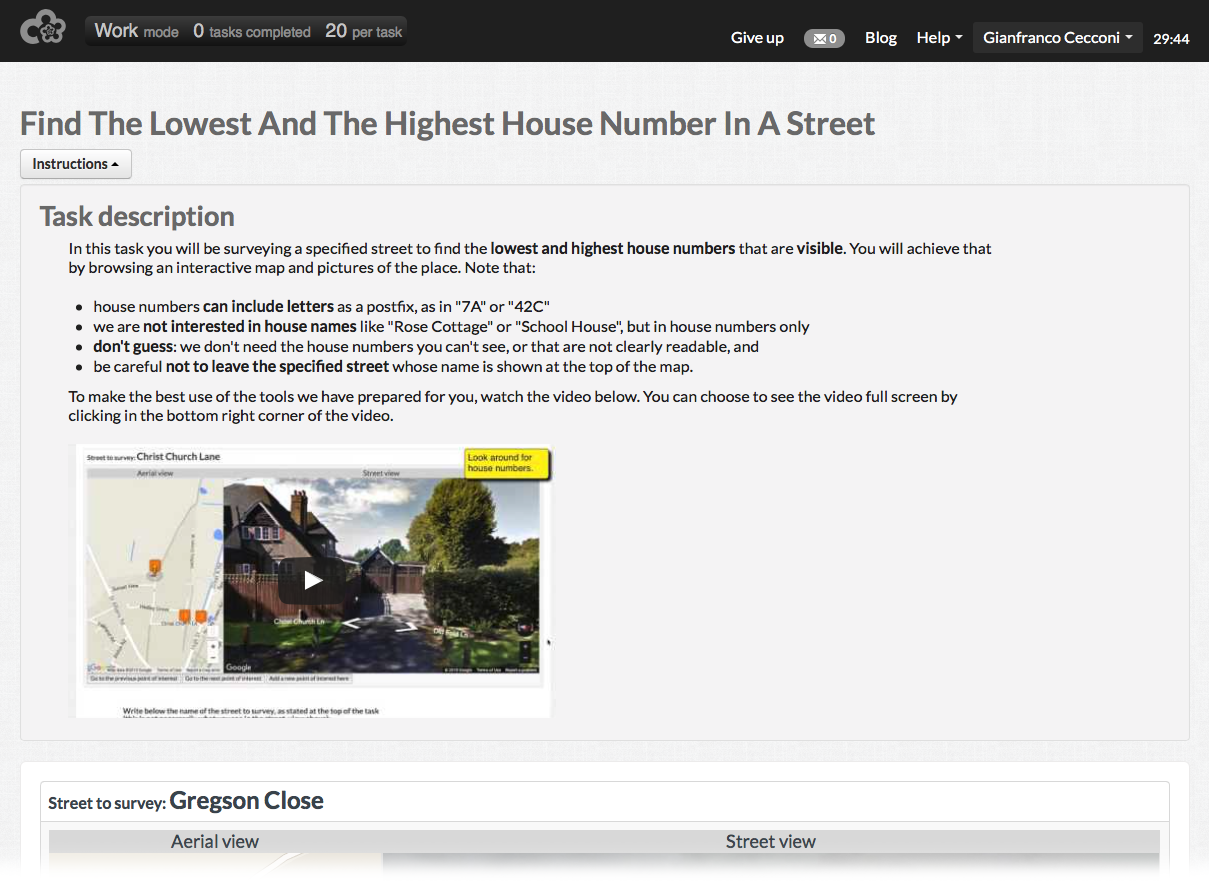
\includegraphics[width=0.49\textwidth]{virtual-survey-tool-02.png}}{\caption{The instruction section of the web page, embedding a video with the instructions.}\label{fig:virtual-survey-tool-02}}
        \ffigbox{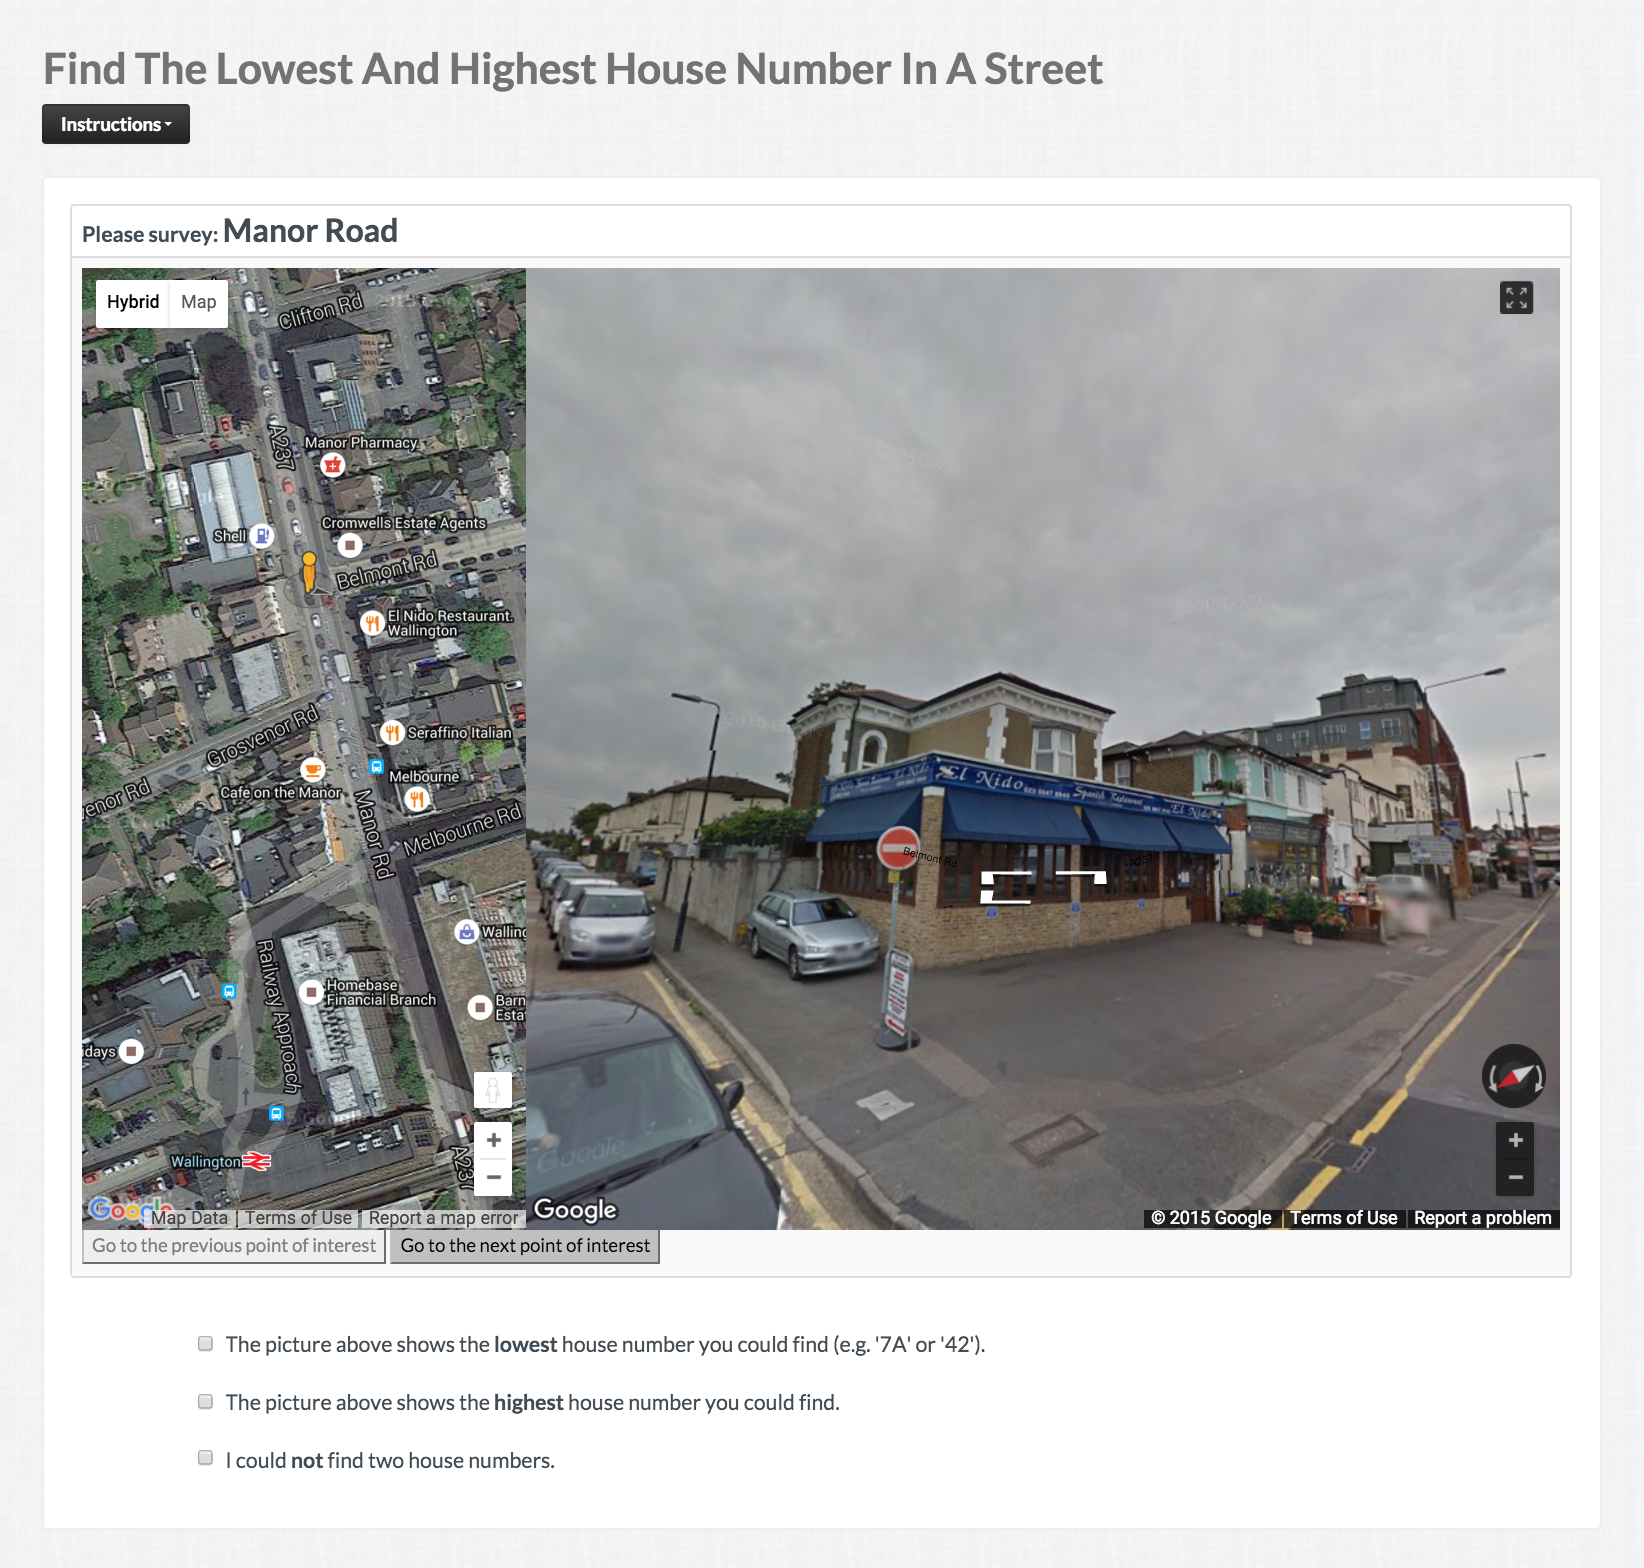
\includegraphics[width=0.49\textwidth]{virtual-survey-tool-01.png}}{\caption{The task section of the web page, offering the Google Maps and Street View panes and the form participants use to submit their observations.}\label{fig:virtual-survey-tool-01}}
    \end{floatrow}
\end{figure}

\subsubsection{Components} \leavevmode \\ %% Why is this necessary to get a new line?

\textbf{CrowdFlower} CrowdFlower was chosen as the crowdsourcing platform. It is a Software-as-a-Service platform specialised in hosting data-centred microtasks for volunteer or paid participants. Clients who accept that their data could be re-published as open data by CrowdFlower may access the service under the "Data for Everyone" plan, that has no costs but for the compensation to the paid participants and a 20\% commission. The service is available both through a templating system called "CrowdFlower Markup Language" (CML) that can be customised by using CrowdFlower's web-based tools, or through APIs. 

When using CML, the options available to implement a crowdsourcing model - such as how the accuracy of the contributor is assessed or how results are aggregated - are limited by the functionality supported by the system\footnote{For example, CrowdFlower calculates the Workers' agreement simply as the \% of participants who expressed the majority vote, and tasks can be stopped automatically when a target agreement \% is achieved. If one wanted to use a stronger statistical tool to calculate agreement, such as Fleiss' Kappa, that automation cannot be used and the calculation must take place outside of the system.}. In order not to introduce additional components in the system and maximise scalability and high availability, it was decided to rely on CML only and work around its limitations by performing some of the tasks outside of CrowdFlower, e.g. results aggregation. 

\textbf{Google Maps} Google Maps is a Software-as-a-Service mapping service for the web and mobile devices, made available by Google to the public for free. It offers satellite and aerial imagery, maps, interactive panoramic views of streets ("Street View") and the respective metadata through APIs. Many of its services can be embedded in third party websites and customised using client-side JavaScript, hence making it very suitable to be integrated with CrowdFlower or any other template-based content management systems. 

It was decided to use Google's mapping services for the prototype as the team had already experience of programming with it. Other equivalent services could have been used as well, e.g. Microsoft's Bing Maps.

\textbf{YouTube} YouTube is a video publishing platform owned by Google. As for Google Maps, videos can be embedded in third party websites, hence YouTube is suitable to be integrated in CrowdFlower's CML templates. The platform uses YouTube to offer participants the instructions video.  

\textbf{PostgreSQL + PostGIS} The PostgreSQL relational database\footnote{See \url{http://www.postgresql.org/}.} running the PostGIS spatial extender \footnote{See \url{http://postgis.net/}.} was chosen as the main data repository for the platform. All geospatial data is converted from its original format (CSV, ESRI Shapefile etc.) to PostGIS' native geospatial types to be consistent across all sources and enabling spatial and geographic querying. When needed, QGIS \footnote{See \url{http://www.qgis.org/}.} was used to quickly visualise the data on maps, e.g. for inspection and debugging.

\textbf{Scripting} Bash, NodeJS and PostgreSQL SQL scripting are used to glue all components together wherever automation is possible.  

\subsubsection{Legal aspects}

The choices made in designing an implementing the platform can have legal implications that need to be taken into account, in particular if the data that is the result of the process is intended to be published under an open licence.

It is outside of the scope of this paper to examine this in detail, although it is useful to present, in the following, some of the issues to consider.

\textbf{Personal data and privacy implications.} According to EU Data Protection Directive (95/46/EC\footnote{See \url{http://eur-lex.europa.eu/LexUriServ/LexUriServ.do?uri=CELEX:31995L0046:en:HTML}.} some geospatial data such as addresses can be considered "personal data" even when it is not associated to information about {\it who} lives at those locations, as it is "information relating to an identified or {\it identifiable} natural person" (no italics in the original). The directive describes a framework of good practices for member states to make into law that we would need to comply with.
	
\textbf{Imagery terms and conditions} Google Maps' terms of service \footnote{See \url{https://www.google.com/intl/en-GB_US/help/terms_maps.html}.} specify a restriction on producing "derivative works of the Content or any part thereof". Moreover, and more specifically, they also include a restriction on using the services to create "a database of places or other local listings information". It can be argued that observing a map or the pictures of a street does not constitute "derivative work". In any case, it is advisable that - before deploying the platform to real-world applications - the mapping services provider is informed and licensing clarified. This is what OpenStreetMap did to integrate Bing imagery\footnote{See \url{http://wiki.openstreetmap.org/wiki/Bing#Bing_Aerial_Imagery}, last accessed 2 January 2016.}.
